\documentclass{standalone}
\usepackage{pgfplots}
\pgfplotsset{compat=1.18}
\newcommand{\point}[2]{\pgfextractx{\dimen0}{\pgfpointanchor{#1}{#2}}\pgfextracty{\dimen2}{\pgfpointanchor{#1}{#2}}\typeout{POINT #1.#2: \the\dimen0,\the\dimen2}}
\begin{document}
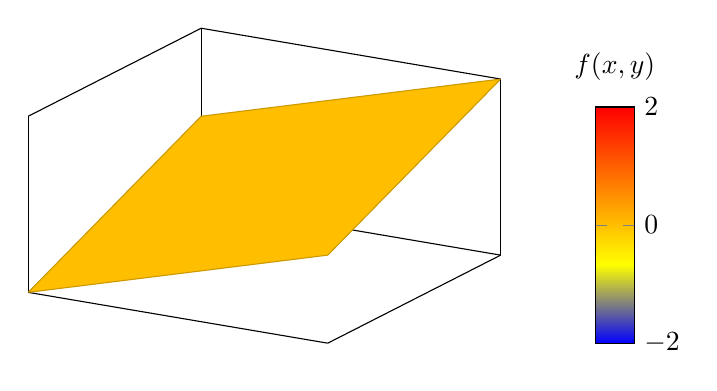
\begin{tikzpicture}
\begin{axis}[scale only axis,width=6cm,height=4cm,view={30}{30},
  enlargelimits=false,xmin=-1,xmax=1,ymin=-1,ymax=1,zmin=-2,zmax=2,
  xtick=\empty,ytick=\empty,ztick=\empty,colorbar,
  colorbar style={name=cb,at={(1.2,0)},anchor=south west,width=.5cm,height=3cm,
    ytick={-2,0,2},yticklabel style={name=tick\ticknum},
    title={$f(x,y)$},title style={name=title}}]
\addplot3[surf,samples=2,domain=-1:1,y domain=-1:1] {x+y};
\end{axis}
\point{cb}{south west}\point{cb}{north east}
\point{tick0}{center}\point{tick1}{center}\point{tick2}{center}
\point{title}{south}\point{title}{center}
\end{tikzpicture}
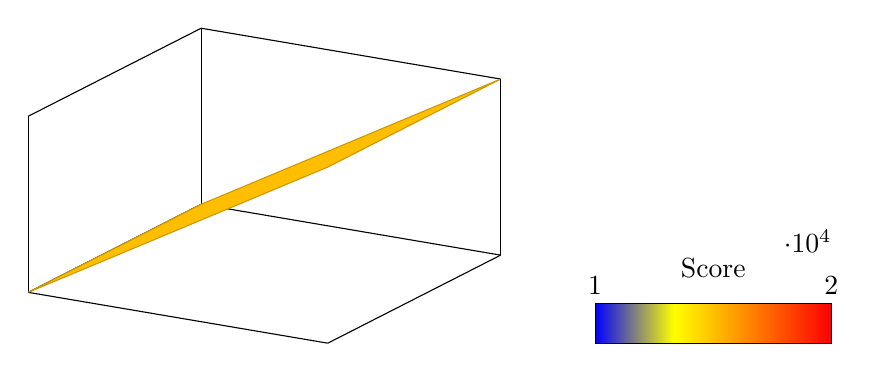
\begin{tikzpicture}
\begin{axis}[scale only axis,width=6cm,height=4cm,view={30}{30},
  enlargelimits=false,xmin=-1,xmax=1,ymin=-1,ymax=1,zmin=10000,zmax=20000,
  xtick=\empty,ytick=\empty,ztick=\empty,colorbar horizontal,
  colorbar style={name=cb,at={(1.2,0)},anchor=south west,width=3cm,height=.5cm,
    xtick={10000,20000},xticklabel pos=upper,xticklabel style={name=htick},
    every x tick scale label/.append style={name=multiplier},
    title={Score},title style={name=title}}]
\addplot3[surf,samples=2,domain=-1:1,y domain=-1:1] {5000*(x+3)};
\end{axis}
\typeout{CASE horizontal}
\point{cb}{south west}\point{cb}{north east}
\point{htick}{center}\point{multiplier}{center}
\point{title}{south}\point{title}{center}
\end{tikzpicture}
\end{document}
